% Author: Izaak Neutelings (September 2020)
% Inspiration: https://tex.stackexchange.com/questions/25531/adding-underbrace-in-tikz
\documentclass[border=3pt,tikz]{standalone}
\usepackage{physics}
\usepackage{ifthen}
\usepackage{tikz}
\usetikzlibrary{patterns}
\tikzset{>=latex} % for LaTeX arrow head

\colorlet{myred}{red!65!black}
\colorlet{acol}{red!50!blue!80!black!80}
\tikzstyle{ground}=[preaction={fill,top color=black!10,bottom color=black!5,shading angle=20},
                    fill,pattern=north east lines,draw=none,minimum width=0.3,minimum height=0.6]
\tikzstyle{mass}=[line width=0.6,red!30!black,fill=red!40!black!10,rounded corners=1,
                  top color=red!40!black!20,bottom color=red!40!black!10,shading angle=20]
\tikzstyle{rope}=[brown!70!black,line width=1.2,line cap=round] %very thick

% FORCES SWITCH
\tikzstyle{force}=[->,myred,thick,line cap=round]
\newcommand{\vbF}{\vb{F}}
\newboolean{showforces}
\setboolean{showforces}{true}


\begin{document}
% NORMAL FORCE lift - acceleration
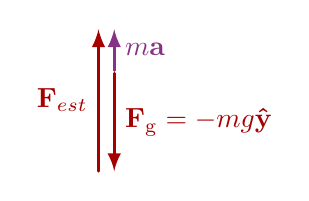
\begin{tikzpicture}
    \def\F{1.8}
    \draw[force,very thick] (0,0) -- (0,\F) node[midway,left=0] {$\vbF_{est}$};
    \draw[force,very thick] (0.2,0.689*\F) --++ (0.0,-0.689*\F) node[midway,right=0] {$\vbF_\mathrm{g}=-mg\vu{y}$};
    \draw[force,acol,very thick] (0.2,0.711*\F) --++ (0.0,0.289*\F) node[midway,right=0] {$m\vb{a}$};
\end{tikzpicture}


\end{document}